\documentclass[11pt]{article}
\usepackage[margin=1in, top=1in]{geometry}
\usepackage[all]{nowidow}
\usepackage[hyperfigures=true, hidelinks, pdfhighlight=/N]{hyperref}
\usepackage[separate-uncertainty=true, group-digits=false]{siunitx}
\usepackage{graphicx,amsmath,physics,tabto,float,amssymb,pgfplots,verbatim,tcolorbox}
\usepackage{listings,xcolor,subfig,caption,import,wrapfig,enumitem}
\usepackage[version=4]{mhchem}
\usepackage[noabbrev]{cleveref}
\newcommand{\creflastconjunction}{, and\nobreakspace}
\definecolor{stringcolor}{HTML}{C792EA}
\definecolor{codeblue}{HTML}{2162DB}
\definecolor{commentcolor}{HTML}{4A6E46}
\captionsetup{font=small, belowskip=0pt}
\lstdefinestyle{appendix}{
    basicstyle=\ttfamily\footnotesize,commentstyle=\color{commentcolor},keywordstyle=\color{codeblue},
    stringstyle=\color{stringcolor},showstringspaces=false,numbers=left,upquote=true,captionpos=t,
    abovecaptionskip=12pt,belowcaptionskip=12pt,language=Python,breaklines=true,frame=single}
\lstdefinestyle{inline}{
    basicstyle=\ttfamily\footnotesize,commentstyle=\color{commentcolor},keywordstyle=\color{codeblue},
    stringstyle=\color{stringcolor},showstringspaces=false,numbers=left,upquote=true,frame=tb,
    captionpos=b,language=Python}
\renewcommand{\lstlistingname}{Appendix}
\pgfplotsset{compat=1.17}

\begin{document}

\begin{center}
    \textbf{CP Tut 2}\hspace{2in}\textbf{KDSMIL001}\hspace{2in}\textbf{30-04-2022}
\end{center}

\begin{enumerate}
    \item Using the Lagrange interpolation method with the Regula Falsi root finding method, we were able to find the root of the function $f(x)=e^x \ln x-x^2$. \\
    To do this, we simply generated data by evaluating $y_i=f(x_i)$ for $x_i=1.0, 1.1, \dots, 2.0$ and then, choosing our starting points as the leftmost and rightmost points of the interval, used linear interpolation to find the $x$-value for which the line connecting the function evaluation at those two points crosses the $x-axis$:
    \begin{align*}
        y(x)&=y_1+\frac{(y_2-y_1)(x-x_1)}{(x_2-x_1)} \overset ! = 0\\
        \implies x&=x_1-y_1\frac{x_2-x_1}{y_2-y_1}
    \end{align*}
    This then replaced the point on the same side of the root as it and we found the function evaluation at that point by interpolation. We ran this algorithm until a tolerance was reached, in our case until the function value at the root was $|y_0|<\num{1e-5}$. 

    \begin{figure}[h]
        \begin{center}
            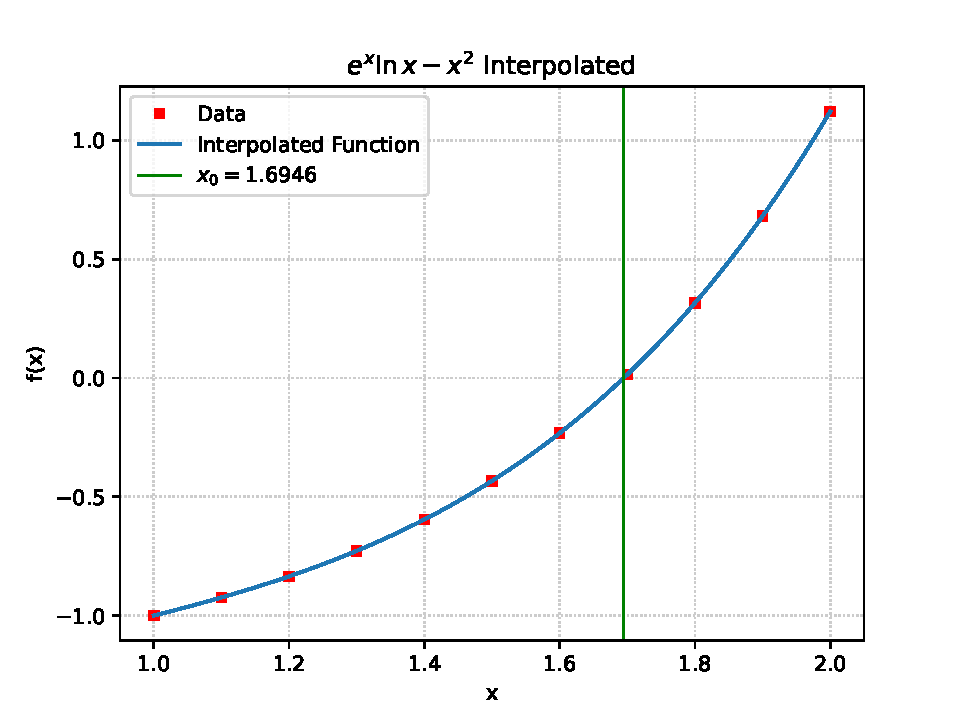
\includegraphics[width=.6\textwidth]{Plots/q1.pdf}
            \caption{Data generated from $y_i=f(x_i)=e^{x_i} \ln(x_i)-x_i^2$ with $x_i=1.0, 1.1, \dots, 2.0$, interpolated using the Lagrange interpolation method on 100 points. The root of the function $x_0$ was found using Regula Falsi and Lagrange interpolation to a tolerance of \num{1e-5}.}
            \label{fig:q1}
        \end{center}
    \end{figure}

    \item In our implementation of Smoothed Particle Interpolation, our two parameters were number of ``particles'' $N$ and smoothing length $h$. We are able to vary $N$ here, but in practice $N$ is most likely going to be fixed as the ``particles'' we choose are most likely going to be the data that we have. \\
    We began by generating our data from the function $f(x)=3x^4-3x^2$ using $N=50$ evenly spaced data points on the interval $[-10,10]$. Since SPI struggles at the boundaries of intervals, we chose to only interpolate over a smaller interval $[-5,5]$. We used the Gaussian kernel function and its derivatives
    \begin{align}
        W(x,x';h) &= \frac{1}{h\sqrt{\pi}}\exp\left(-\left(\frac{x'-x}{h}\right)^2\right) \label{eqn:GaussianKernel}\\
        W'(x,x';h) &= \frac{-2(x'-x)}{h^3\sqrt{\pi}}\exp\left(-\left(\frac{x'-x}{h}\right)^2\right) \label{eqn:GaussianKernelPrime}\\
        W''(x,x';h) &= \frac{-2}{h^3\sqrt{\pi}}\exp\left(-\left(\frac{x'-x}{h}\right)^2\right) + \frac{4(x'-x)^2}{h^5\sqrt{\pi}}\exp\left(-\left(\frac{x'-x}{h}\right)^2\right) \label{eqn:GaussianKernelPrimePrime}
    \end{align}
    where $x$ is the point at which we evaluate the function, $x'$ are the data points, which we sum over for each $x$, and $h$ is the smoothing length, i.e. the width of the Gaussian. Using these, the interpolation for the function and its first 2 derivatives was 
    \begin{align}
        f(x)&\approx \sum_i \Delta x_i f(x_i) W(x,x_i;h) \label{eqn:SPI}\\
        f'(x)&\approx -\sum_i \Delta x_i f(x_i) W'(x,x_i;h) \label{eqn:SPIPrime}\\
        f''(x)&\approx \sum_i \Delta x_i f(x_i) W''(x,x_i;h) \label{eqn:SPIPrimePrime}
    \end{align}
    where the $x_i$ are our data points, or ``particles''.\\
    With these approximations, using $N=50$ and $h=0.5$, we found were able to interpolate 1 000 points on the interval $[-5,5]$ and get the plots in \cref{fig:q2afunc}. These can be compared to the exact values of the function and its derivatives in \cref{fig:q2aexact}.

    \begin{figure}[h]
        \begin{center}
            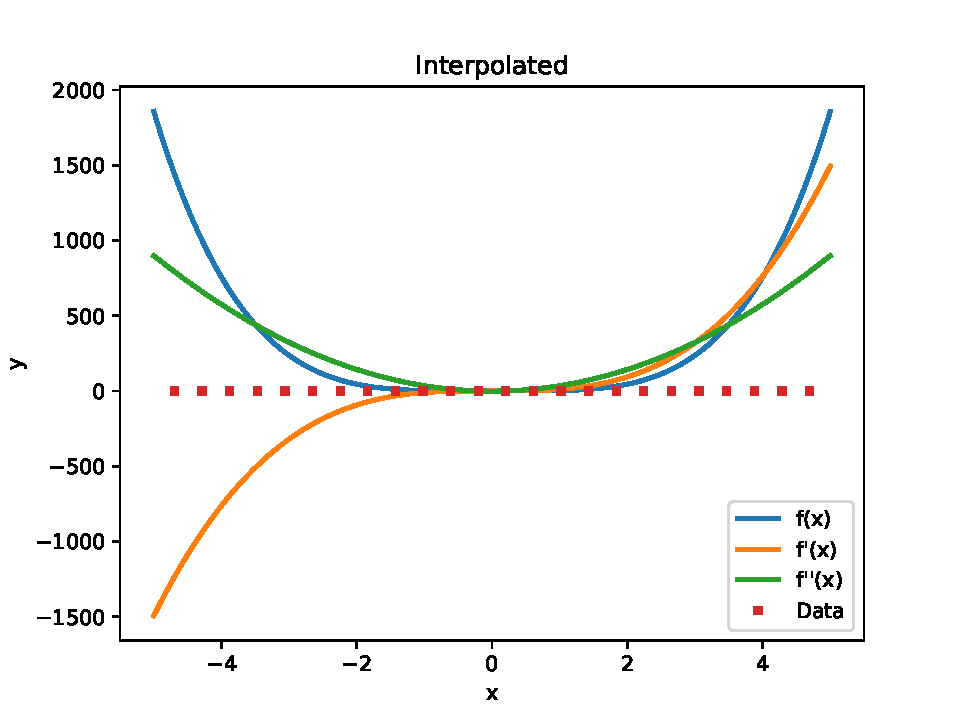
\includegraphics[width=.6\textwidth]{Plots/q2afunc.pdf}
            \caption{Data generated from $y_i=f(x_i)=3x_i^4-3x_i^2$ with $x_i\in[-10,10]$, interpolated using SPI on 1 000 points in the interval $[-5,5]$ to find the function value as well as its first two derivatives.}
            \label{fig:q2afunc}
        \end{center}
    \end{figure}
    
    \begin{figure}[h]
        \begin{center}
            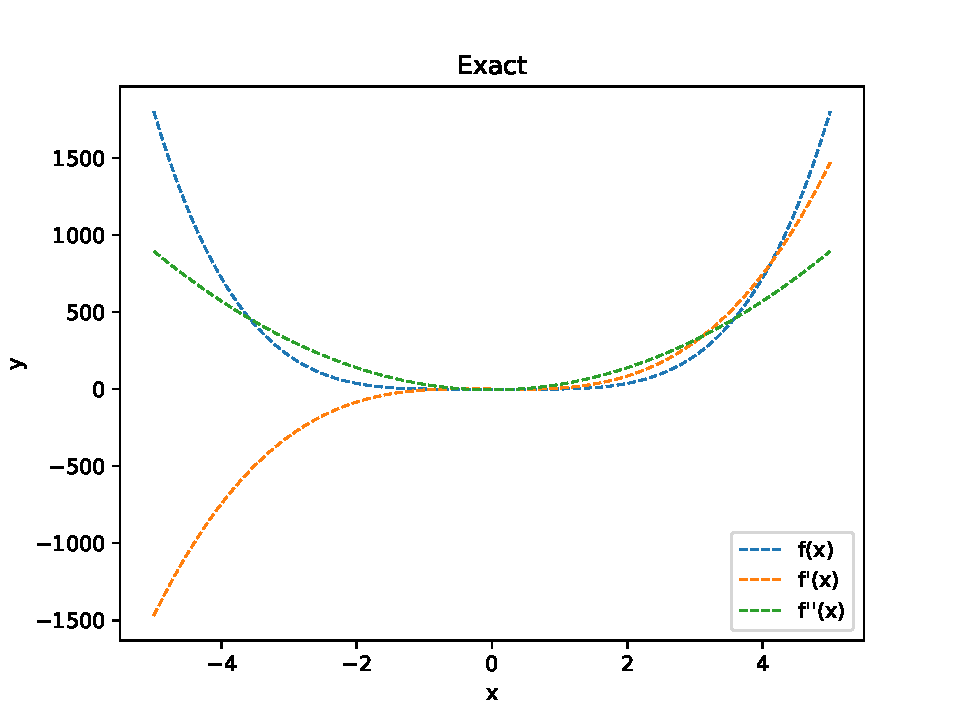
\includegraphics[width=.6\textwidth]{Plots/q2aexact.pdf}
            \caption{The exact form of the function $f(x)=3x^4-3x^2$ and its first two derivatives, evaluated on 1 000 points in the interval $[-5,5]$.}
            \label{fig:q2aexact}
        \end{center}
    \end{figure}
    
    What is of interest is the error between the interpolated functions and the exact value, so plotted in \cref{fig:q2a1,fig:q2a2,fig:q2a3} is the difference between the interpolated values and the exact values, for the function and its first two derivatives.

    \begin{figure}[h]
        \begin{center}
            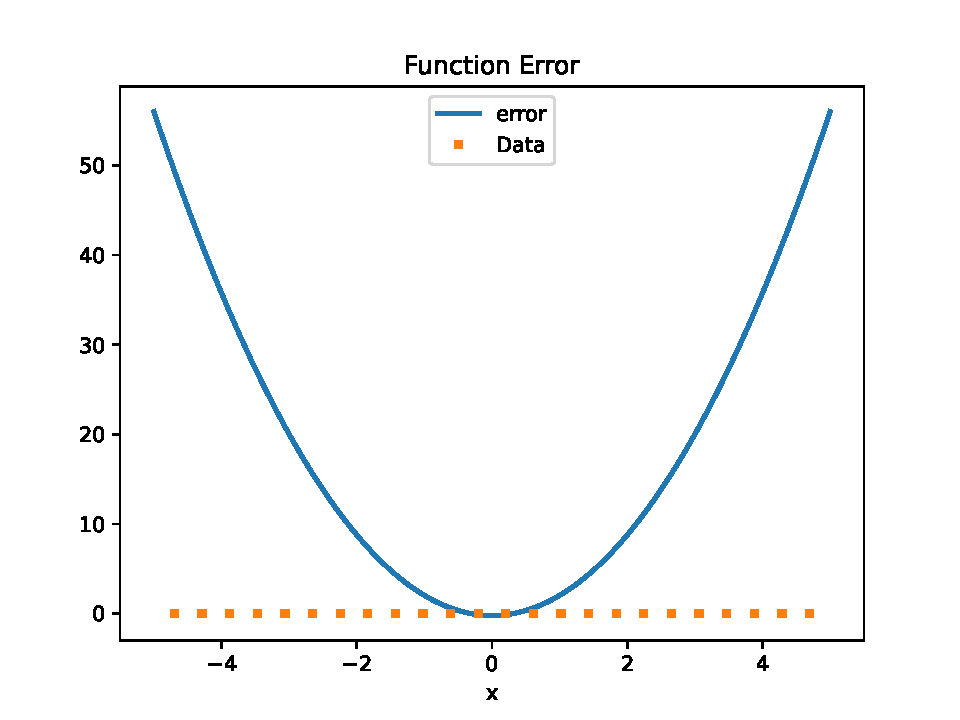
\includegraphics[width=.6\textwidth]{Plots/q2a1.pdf}
            \caption{Error between the interpolated values and the exact values for $f(x)=3x^4-3x^2$ on 1 000 points in the interval $[-5,5]$.}
            \label{fig:q2a1}
        \end{center}
    \end{figure}

    \begin{figure}[h]
        \begin{center}
            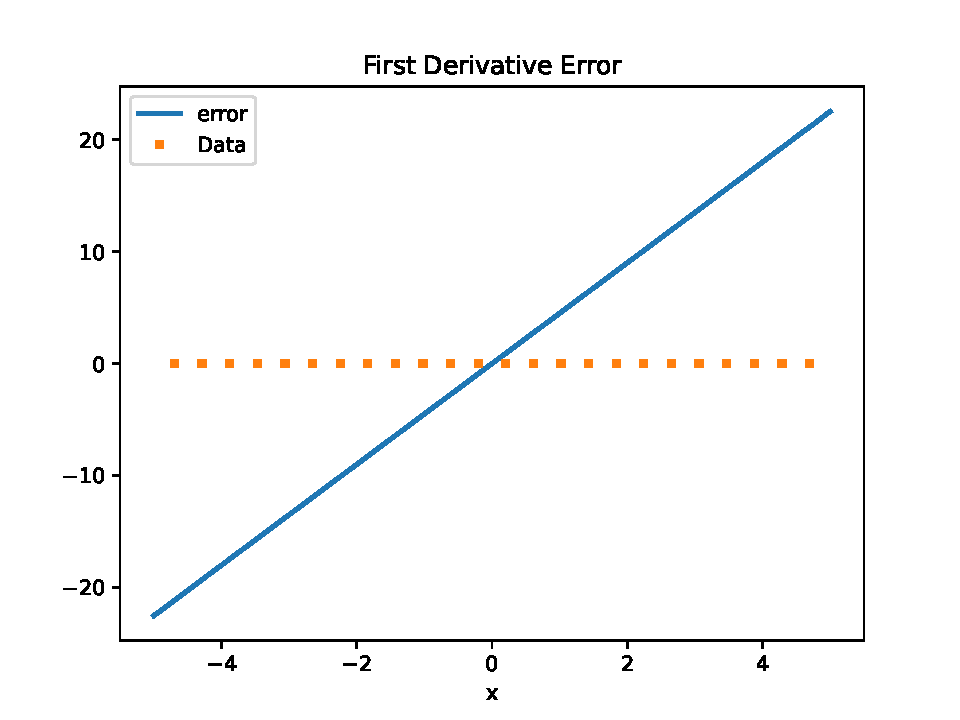
\includegraphics[width=.6\textwidth]{Plots/q2a2.pdf}
            \caption{Error between the interpolated values and the exact values for $f'(x)=12x^3-6x$ on 1 000 points in the interval $[-5,5]$.}
            \label{fig:q2a2}
        \end{center}
    \end{figure}

    \begin{figure}[h]
        \begin{center}
            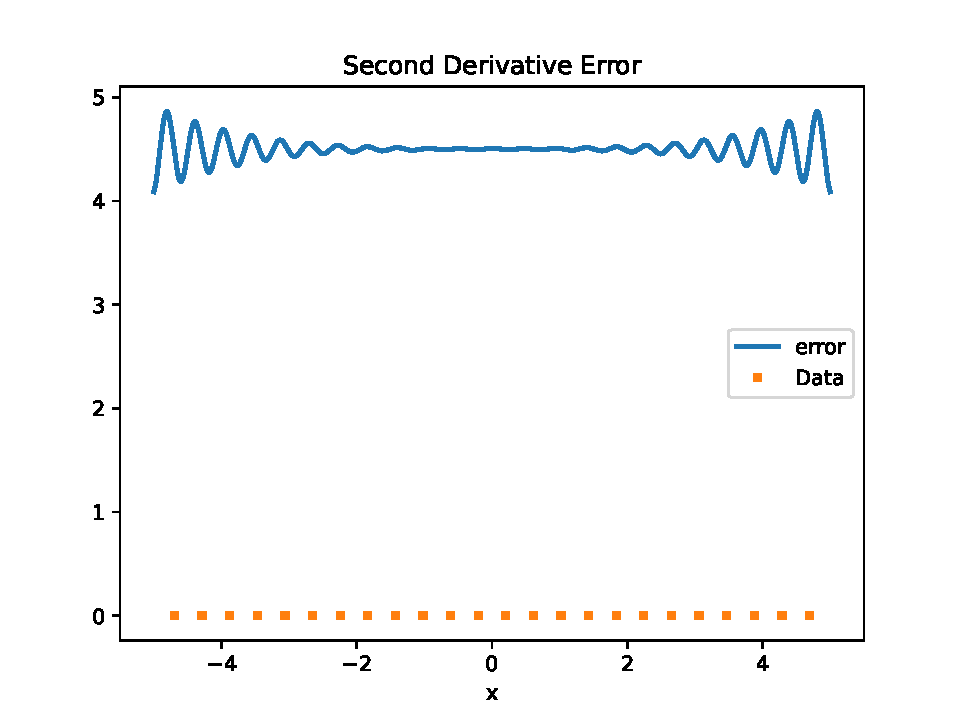
\includegraphics[width=.6\textwidth]{Plots/q2a3.pdf}
            \caption{Error between the interpolated values and the exact values for $f''(x)=36x^2-6$ on 1 000 points in the interval $[-5,5]$.}
            \label{fig:q2a3}
        \end{center}
    \end{figure}
    

\end{enumerate}

\end{document}